\subsection{\textit{Optimized link state routing} - OLSR}
O protocolo OLSR \cite{rfc3626} \'e um protocolo pr\'o-ativo, baseado em estado de conex\~ao, onde cada n\'o possui as informa\c{c}\~oes de rotas e compartilham entre si constantemente. 
O diferencial desse protocolo em rela\c{c}\~ao ao DSDV, que tamb\'em \'e pro-\'ativo, por\'em baseado em dist\^ancia de vetores, \'e que o OLSR diminui o tr\'afego de informa\c{c}\~oes de roteamento utilizando somente alguns n\'os pr\'e-selecionados, para retransmitir as mensagens de descoberta de rotas na rede.
Essa t\'ecnica \'e denominada MPR (\textit{Multipoint Relay}).

\subsubsection{Exemplo de funcionamento do OLSR}
Considerando as Figuras \ref{fig:olsrComum} e \ref{fig:olsrOperation}, temos a diferen\c{c}a de funcionamento de descoberta de rotas a cada passo, onde cada n\'o repassa as informa\c{c}\~oes de rotas entre os n\'os vizinhos.

\begin{figure}[H]
	\centering
	\subfigure[Primeiro est\'agio]{
		\includegraphics[scale=0.3]{olsrOperationStep1.eps}
	}\label{subfig:olsrStep11}
	\subfigure[Segundo est\'agio]{
		\includegraphics[scale=0.3]{olsrOperationStep2.eps}
	}\label{subfig:olsrStep12}
	\subfigure[Terceiro est\'agio]{
		\includegraphics[scale=0.3]{olsrOperationStep3.eps}
	}\label{subfig:olsrStep13}
	\subfigure[Quarto est\'agio]{
		\includegraphics[scale=0.3]{olsrOperationStep4.eps}
	}\label{subfig:olsrStep14}	
	\caption{Descoberta de rotas do protocolo DSDV}
	\label{fig:olsrComum}
\end{figure}

O mecanismo para selecionar os vizinhos que ir\~ao retransmitir os pacotes, denominado MPR, \'e simples. Ele escolhe vizinhos alcan\c{c}\'aveis atrav\'es de um salto que tenham comunica\c{c}\~ao sim\'etrica, bidirecional, com pacotes de mensagens \textit{HELLO}

\begin{figure}[H]
	\centering
	\subfigure[Primeiro est\'agio]{
		\includegraphics[scale=0.3]{olsrOperationStep1.eps}
	}\label{subfig:olsrStep21}
	\subfigure[Segundo est\'agio]{
		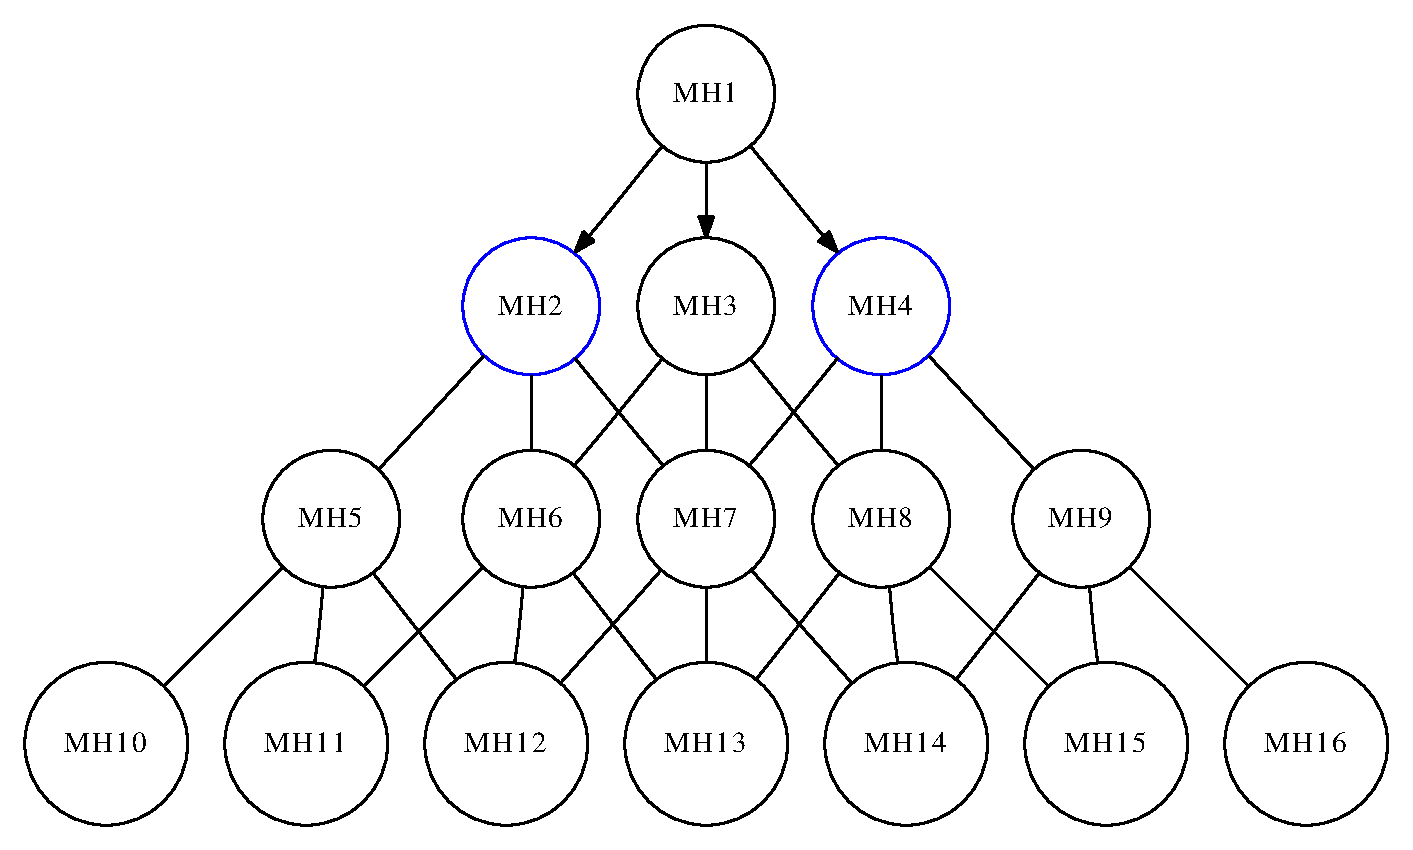
\includegraphics[scale=0.3]{olsrOperationStep5.eps}
	}\label{subfig:olsrStep22}
	\subfigure[Terceiro est\'agio]{
		\includegraphics[scale=0.3]{olsrOperationStep6.eps}
	}\label{subfig:olsrStep23}
	\subfigure[Quarto est\'agio]{
		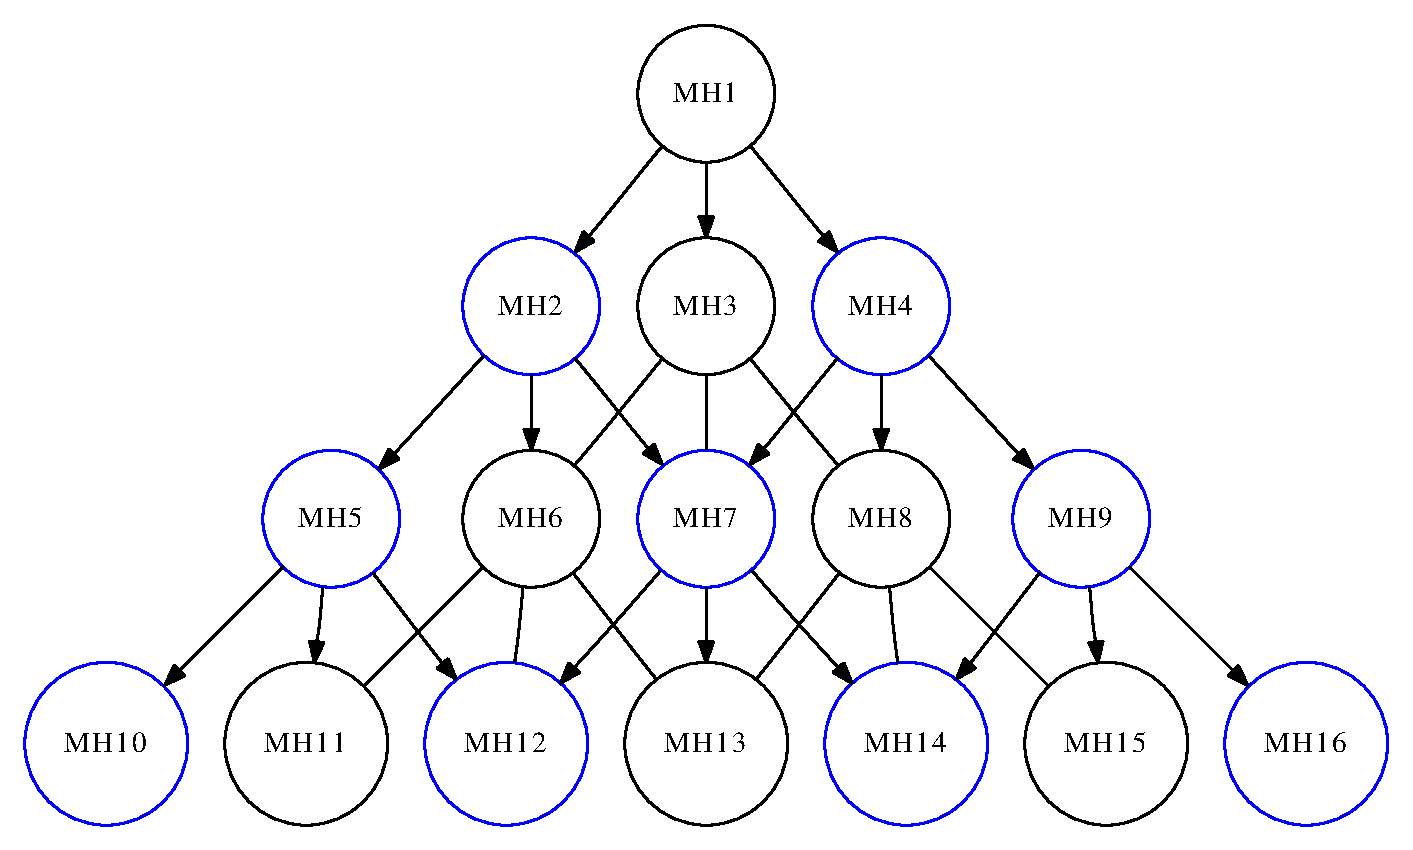
\includegraphics[scale=0.3]{olsrOperationStep7.eps}
	}\label{subfig:olsrStep24}	
	\caption{Descoberta de rotas do protocolo OLSR}
	\label{fig:olsrOperation}
\end{figure}


